\documentclass[11pt,a4paper]{article}

% Full step-by-step report of everything done so far (27 October 2026).
% Figures: full_report_figures.pdf, one figure per page, made by latex/full_report/figures.py
% from the data in the repository. Bibliography: references.bib (shared with the proposal).

\usepackage[utf8]{inputenc}
\usepackage[T1]{fontenc}
\usepackage{lmodern}
\usepackage[margin=2.5cm]{geometry}
\usepackage{microtype}
\usepackage{amsmath,amssymb}
\usepackage{booktabs}
\usepackage{tabularx}
\usepackage{longtable}
\usepackage{array}
\usepackage{enumitem}
\usepackage{graphicx}
\usepackage[table]{xcolor}
\usepackage{textcomp}
\usepackage[most]{tcolorbox}
\usepackage[section]{placeins}
\usepackage[authoryear,round]{natbib}
\usepackage[colorlinks=true,linkcolor=blue!50!black,citecolor=blue!50!black,urlcolor=blue!50!black]{hyperref}

\setlist{itemsep=2pt,topsep=4pt}
\setlength{\parskip}{3pt}
\newcolumntype{L}{>{\raggedright\arraybackslash}X}
\newcolumntype{P}[1]{>{\raggedright\arraybackslash}p{#1}}

% one figure per page of this PDF
\newcommand{\fig}[2][\textwidth]{\includegraphics[page=#2,width=#1]{full_report_figures.pdf}}

\definecolor{boxblue}{HTML}{EEF3FB}
\definecolor{boxline}{HTML}{2A78D6}
\definecolor{trgrey}{HTML}{F4F4F1}
\definecolor{trline}{HTML}{898781}
\definecolor{donecol}{HTML}{1BAF7A}
\definecolor{probcol}{HTML}{EB6834}
\definecolor{nextcol}{HTML}{2A78D6}

% a key message
\newtcolorbox{keybox}[1][]{breakable, colback=boxblue, colframe=boxline, boxrule=0pt, leftrule=3pt,
  arc=0pt, left=8pt, right=8pt, top=4pt, bottom=4pt, fonttitle=\bfseries, coltitle=black,
  title={#1}, attach title to upper={\ }, before skip=8pt, after skip=8pt}
% literal model text
\newtcolorbox{transcript}[1][]{breakable, colback=trgrey, colframe=trline, boxrule=0pt, leftrule=2pt,
  arc=0pt, left=8pt, right=8pt, top=4pt, bottom=4pt, fontupper=\small, fonttitle=\small\bfseries,
  coltitle=black, title={#1}, attach title to upper={\par\smallskip}, before skip=8pt, after skip=8pt}
\newcommand{\who}[1]{\par\smallskip\noindent\textsf{\textbf{\footnotesize\MakeUppercase{#1}}}\quad}
\newcommand{\cut}{\textup{[\dots]}}

% done / problem / next step summary at the end of each step
\newcommand{\dpn}[3]{%
\begin{tcolorbox}[breakable, colback=white, colframe=trline, boxrule=0.4pt, arc=0pt, left=6pt, right=6pt, top=4pt, bottom=4pt, before skip=10pt, after skip=10pt]
\small
\noindent{\color{donecol}\textsf{\textbf{DONE}}}\quad #1\par\medskip
\noindent{\color{probcol}\textsf{\textbf{PROBLEM}}}\quad #2\par\medskip
\noindent{\color{nextcol}\textsf{\textbf{WHAT WE DID / DO NEXT}}}\quad #3
\end{tcolorbox}}

\title{\textbf{Anchoring in Large Language Models}\\[4pt]
\large Everything we have done so far, step by step\\[2pt]
\normalsize Project: \emph{Adjusting or Retrieving? Testing the Mechanisms of Anchoring in Large Language Models}}
\author{Hannan Seyfi\\[6pt]
\normalsize Supervisors: Dr.\ Shiva Kamkar and Dr.\ Babak Majidi\\
\normalsize Khatam University}
\date{27 October 2026}

\begin{document}
\maketitle

\begin{keybox}[The project in three sentences.]
When a language model sees a number before it estimates something, its estimate moves towards that number. This is called \emph{anchoring}, and it is well known in people and already shown in language models. We want to find out \emph{why} it happens in models, by testing the two explanations that psychology offers for people, and by reading the model's own thinking as it answers.
\end{keybox}

\begin{keybox}[Where we are on 27 October 2026.]
We have written the proposal, built all the software, run two pilot runs (a small 1.5-billion-parameter model and the 32-billion-parameter Qwen3-32B), learned that the large model already knew our first questions, written 299 new candidate questions, screened them, and picked 15 new questions for Study~1 and 10 for Study~2. The next step is to run the pilot again on these new questions. Altogether we have collected 38,320 model answers for \$2.93.
\end{keybox}

\paragraph{How to read this report.} Part~I explains the idea from zero. Part~II explains the tools we built. Part~III goes through every step we took, in order, with real questions, the model's real answers and real thinking, and a figure for each result. Every step ends with a box that says what was \textcolor{donecol}{\textbf{done}}, what \textcolor{probcol}{\textbf{problem}} we found, and what we \textcolor{nextcol}{\textbf{did or will do}} about it. Part~IV collects everything into one long list and a plan. Words that may be new are explained in the glossary (Appendix~\ref{app:glossary}). Text in grey boxes is copied exactly from the model, including its mistakes; \cut{} marks where we left text out.

\tableofcontents
\clearpage

% =====================================================================
\part{The idea}
% =====================================================================

\section{Introduction from zero}
\label{sec:intro}

\subsection{What is anchoring?}

Imagine someone asks you two questions:
\begin{enumerate}
  \item Is the height of Angel Falls in Venezuela more or less than 11,000 metres?
  \item How tall do you think Angel Falls is?
\end{enumerate}
The first question gives you a number, 11,000\,m. It is far too high (the real height is 979\,m), and you know it is only part of the question, not a hint. Still, people who get a high number in the first question give higher answers to the second question than people who get a low number. The first number is called the \textbf{anchor}, and the pull of the answer towards it is called \textbf{anchoring}.

The classic demonstration is by \citet{tversky1974judgment}. People watched a wheel of fortune stop at 10 or at 65, then estimated the percentage of African countries in the United Nations. The wheel was obviously random. People who saw 10 gave a median estimate of 25\%; people who saw 65 gave 45\%. Kahneman made this a central example of fast, intuitive ``System~1'' thinking in his book \emph{Thinking, Fast and Slow} \citep{kahneman2011thinking}, which is where this project started.

\subsection{Why it matters for language models}

Large language models (LLMs) such as ChatGPT, Claude, Qwen and DeepSeek are now asked for numbers all the time: prices, forecasts, medical doses, grades for essays, estimates in reports. The text they read often contains numbers that should not matter (an earlier guess, a number in a document, a score from another grader). If these numbers pull the model's answer, that is a practical problem. Many recent papers show that LLMs do anchor, often more strongly than people \citep{lou2026anchoring,huang2025understanding,borjigin2026anchorbench}.

\subsection{Two explanations from psychology}
\label{sec:two}

Psychologists have two main explanations for \emph{why} people anchor (Figure~\ref{fig:mech}).

\begin{figure}[ht]
\centering
\fig{1}
\caption{The two explanations, drawn as a number line. The shaded band is the range of values the model (or person) finds plausible without an anchor; the grey dots are answers without an anchor. \textbf{A, adjusting:} the answer starts at the anchor and moves towards the plausible values in small steps, but stops too early, at the edge of the band. \textbf{B, retrieving:} the anchor does not set a starting point; it changes \emph{which} memory comes to mind. Some answers are the usual one, others are a value that fits the anchor.}
\label{fig:mech}
\end{figure}

\paragraph{Explanation 1: Adjusting (``insufficient adjustment'').} You start from the anchor and adjust away from it until the answer seems reasonable. But you stop too early, at the first value that seems acceptable, which is the edge of the range you find plausible \citep{tversky1974judgment,epley2006anchoring}.
\emph{Everyday example:} you are told a used car costs \$20,000. You think ``too much'', lower it to \$17,000, then \$15,000, and stop at the first price that feels fair. If you had started from \$10,000, you would have stopped lower.

\paragraph{Explanation 2: Retrieving (``selective accessibility'').} When you ask yourself ``is it 11,000\,m?'', you search your memory for things that \emph{fit} 11,000\,m (``it is the tallest waterfall in the world'', ``it falls from a huge mountain''). These facts are now easier to recall, and they shape your final answer \citep{strack1997explaining,mussweiler1999hypothesis}. There is no starting point and no adjustment; the anchor changes \emph{what information you use}.
\emph{Everyday example:} if someone asks whether a city has more than 10 million people, you start thinking of its traffic, its skyscrapers and its suburbs, and your estimate rises.

\paragraph{Why the difference matters.} The two explanations suggest different cures. If anchoring is adjusting that stops too early, then \emph{more thinking} should help: you keep adjusting. If anchoring is retrieving, more thinking can make it \emph{worse}, because you retrieve more anchor-consistent facts; the cure is to ``consider the opposite'', that is, to look for reasons why the anchor is wrong \citep{mussweiler2000overcoming}.

\subsection{Who supplies the anchor?}
\label{sec:selfgiven}

\citet{epley2001putting} found that both explanations are right, but for different kinds of anchors.
\begin{itemize}
  \item A \textbf{self-generated} anchor is one you think of yourself. Example: ``At what temperature does water boil on the top of Mount Everest?'' Most people start from 100\,\textdegree C (sea level), which they know, and adjust downwards. People described this adjusting when asked to think aloud, and extra effort (being paid for accuracy, being warned) moved their answers further.
  \item A \textbf{provided} (given) anchor is one somebody else gives you, as in the Angel Falls question above. Here people rarely described adjusting, and extra effort did not help \citep{epley2005effortful}.
\end{itemize}
So in people, \emph{more effort helps only when you chose the anchor yourself}.

\subsection{Why we can study this now}

Two recent developments make the question answerable for LLMs.
\begin{enumerate}
  \item \textbf{Reasoning models show their thinking.} Models such as DeepSeek-R1 and Qwen3 write out their reasoning before they answer \citep{guo2025deepseek,yang2025qwen3}. We can read whether a model starts at the anchor and adjusts, or whether it recalls facts that fit the anchor. This is like the ``think aloud'' reports used with people.
  \item \textbf{A puzzling result.} \citet{kraishan2026long} found that giving models a bigger thinking budget did \emph{not} reduce anchoring. But they used only provided anchors, and only five questions. From the human research we would expect exactly this for provided anchors, and we would expect the opposite for self-generated anchors. Nobody has tested that.
\end{enumerate}

\subsection{Our research questions}

\begin{description}[leftmargin=1.2cm,labelwidth=1cm]
  \item[RQ1] When a model is given an anchor, does it behave like adjusting or like retrieving?
  \item[RQ2] Does the model treat self-generated and provided anchors differently, as people do?
  \item[RQ3] Does more thinking reduce anchoring for self-generated anchors but not for provided ones?
  \item[RQ4] Which cure works for which anchor: more thinking, an accuracy instruction, or ``consider the opposite''?
\end{description}

\subsection{What others have already done, and the gap}

Table~\ref{tab:lit} lists the closest papers. They show \emph{that} models anchor, \emph{how strongly}, \emph{through which channels}, and \emph{where in the network}. None tests \emph{which mechanism} produces it, and none compares self-generated with provided anchors in the sense of \citet{epley2001putting}. The two closest papers (SynAnchors and AnchorBench) were read in full on 20 October 2026; the others only at abstract level so far.

\begin{table}[ht]
\centering\small
\begin{tabularx}{\textwidth}{@{}P{3.6cm}L@{}}
\toprule
\textbf{Paper} & \textbf{What it found} \\
\midrule
\citet{lou2026anchoring} & GPT-3.5/4/4o anchor strongly; chain-of-thought, reflection and ``ignore the hint'' do not fix it. \\
\citet{huang2025understanding} (SynAnchors) & 11 models; 22--61\% of questions anchored; reasoning models least affected; selective accessibility mentioned only as an analogy. \\
\citet{owusu2026anchoring} & Less confident models anchor more; high anchors pull more than low ones. \\
\citet{owusu2026localizing} & Finds the internal pathways that carry anchoring in 7--8B models. \\
\citet{borjigin2026anchorbench} (AnchorBench) & Anchors enter through prompts, chat history, documents and tools; ``self-generated'' there means the model's own earlier answer. \\
\citet{kapetanovic2026anchoring} & LLM graders are biased by earlier scores. \\
\citet{kraishan2026long} & A bigger thinking budget does not reduce anchoring (5 provided-anchor questions). \\
\bottomrule
\end{tabularx}
\caption{Closest earlier work. The full table with more detail is in the proposal.}
\label{tab:lit}
\end{table}

\dpn{Literature search and gap analysis (20 October 2026); research direction chosen with the professors' interest in mind; the two closest papers read in full.}
{Most papers are read only at abstract level. The field moves fast: a paper testing the mechanism could appear.}
{Read the remaining papers in full before writing the paper's related-work section, and search again for new papers just before submission.}

% =====================================================================
\section{The plan: what the proposal says}
\label{sec:proposal}
% =====================================================================

The proposal (written in Overleaf on 20 October 2026, 10 pages, file \texttt{main.tex}) plans a pilot and two studies.

\subsection{Study 1: provided anchors}

We ask a question with a provided anchor in the classic two-step form \citep{jacowitz1995measures}: first ``is it higher or lower than $X$?'', then ``give your best estimate''. The anchors are placed \emph{relative to each model's own answers}:
\begin{enumerate}
  \item First we ask each question without an anchor many times (the \textbf{baseline}). The middle of these answers is the model's \textbf{normal zone} (also called its plausible range).
  \item Then we place eight anchors per question: \textbf{low or high} (below or above the zone) $\times$ \textbf{near or far} (just outside the zone, or far outside it) $\times$ \textbf{round or precise} (11,000 or 11,180).
\end{enumerate}
Figure~\ref{fig:design} shows the eight anchors for Angel Falls in the first pilot run.

\begin{figure}[ht]
\centering
\fig{2}
\caption{Where the anchors go, using Angel Falls in pilot run 1. The shaded band is the small model's normal zone (310 to 5,555\,m). Near anchors sit just outside it, far anchors much further out. Each round anchor also has a precise twin (11,000 and 11,180; 99,000 and 100,700). The axis is logarithmic: each step is ten times bigger than the one before.}
\label{fig:design}
\end{figure}

\paragraph{Why near and far?} This is the main test between the two explanations.
\begin{itemize}
  \item If the model \textbf{adjusts}, it stops at the edge of its normal zone. A far anchor then pulls no further than a near one, because the answer stops at the same edge.
  \item If the model \textbf{retrieves}, the whole set of answers moves towards the anchor by a similar share. A far anchor then pulls further than a near one.
\end{itemize}

\paragraph{Why round and precise?} In people, precise anchors (4,988) pull harder than round ones (5,000), which is explained by adjusting in smaller steps from a precise number \citep{janiszewski2008precision}.

\subsection{Study 2: self-generated vs provided anchors}

Each question has a familiar but wrong starting value, called the \textbf{reference value} $R$. Example: ``What is the normal body temperature of a healthy adult chicken?'' The familiar value is $R=37$\,\textdegree C (a human's temperature); the true value is 41.5\,\textdegree C.
\begin{itemize}
  \item \textbf{Self:} we just ask the question. The model has to think of 37\,\textdegree C by itself.
  \item \textbf{Provided:} we ask ``is it higher or lower than 37\,\textdegree C?'' first.
\end{itemize}
Each version is asked with no instruction, with an accuracy instruction, and with a ``consider the opposite'' instruction, at three thinking levels. The human prediction: more thinking helps in the self condition but not in the provided condition (RQ3).

\subsection{How we measure}
\label{sec:measures}

\paragraph{Anchoring index} \citep{jacowitz1995measures}. How far apart are the answers after a high and a low anchor, compared with how far apart the anchors are?
\[
\text{anchoring index} = \frac{\text{median answer after high anchor} - \text{median answer after low anchor}}{\text{high anchor} - \text{low anchor}}
\]
\emph{Worked example} (Angel Falls, pilot run 1): the near anchors were 11,000 and 150\,m, and the median answers were 10,414 and 322\,m. So the index is $(10{,}414 - 322)/(11{,}000-150) = 10{,}092/10{,}850 = 0.93$. An index of 0 means the anchor changed nothing; 1 means the answers moved as far as the anchors. People typically score 0.4 to 0.6; the classic study found 0.49.

\paragraph{Shift.} How far the median answer moved from the model's usual answer towards the anchor, on a log scale: 0 = no movement, 1 = the answer equals the anchor. For Angel Falls (low thinking), the near anchor gave a shift of 0.98 and the far anchor 0.08.

\paragraph{Adjustment} (Study 2). How far the answer moved from the reference value $R$ towards the truth $T$:
\[
\text{adjustment} = \frac{\text{median answer} - R}{T - R}.
\]
\emph{Worked example} (chicken): $R = 37$, $T = 41.5$. A median answer of 37 gives 0 (stayed at the start), 41.5 gives 1 (reached the truth), and 39.25 gives 0.5 (half way). An answer of 35.5 gives $-0.33$: it moved the \emph{wrong} way.

\paragraph{Thinking tokens.} How many words (tokens) the model actually wrote in its thinking. We count them for every answer, because a model may stop thinking long before its budget runs out.

\paragraph{Reading the traces.} We read the model's thinking and code what it does: adjusting (starts at the anchor and moves away step by step), retrieving (collects facts that fit the anchor), dismissing the anchor, or not engaging with it.

\subsection{What each explanation predicts}

\begin{table}[ht]
\centering\small
\begin{tabularx}{\textwidth}{@{}P{3.4cm}LL@{}}
\toprule
\textbf{Signature} & \textbf{Adjusting} & \textbf{Retrieving} \\
\midrule
Where anchored answers land & Pile up at the edge of the normal zone nearest the anchor & The whole set of answers moves towards the anchor \\
Near vs far anchor & Far pulls no further than near & Far pulls further \\
Precise vs round & Precise pulls harder & No difference \\
More thinking or ``be accurate'' & Less anchoring & No less, maybe more \\
``Consider the opposite'' & Little effect & Less anchoring \\
The thinking text & Starts at the anchor, steps away & Lists facts that fit the anchor \\
\bottomrule
\end{tabularx}
\caption{The signatures that tell the two explanations apart (from the proposal).}
\label{tab:pred}
\end{table}

\paragraph{Hypotheses.} From the human research we expect: provided anchors look like retrieving (H1); self-generated anchors look like adjusting (H2); more thinking helps for self-generated anchors only (H3); ``consider the opposite'' helps more for provided anchors (H4). If models show something else, that is also a finding: they reproduce the human \emph{outcome} through a different process.

\dpn{Proposal written in Overleaf (\texttt{main.tex}, 10 pages, compiles cleanly), copy in the repository at \texttt{latex/proposal/}. Research questions, design, measures, predictions, timeline and risks are all written down.}
{The proposal plans about 80 Study~1 and 60 Study~2 questions and about five models. The pilot has since shown that good questions are much harder to find than planned (Part~III).}
{Update the proposal's methods after the v2 pilot: the screening step, the new Study~2 question types, and the size ladder of Qwen3 models.}

% =====================================================================
\part{The tools we built}
% =====================================================================

\section{How one experiment works}
\label{sec:pipeline}

Everything lives in the GitHub repository \texttt{HannanSeyfi/Anchoring-LLMs}. Experiments run in Google Colab notebooks that open from GitHub and save their results back to GitHub. Appendix~\ref{app:files} lists every folder.

\subsection{The steps of a run}

\begin{enumerate}
  \item \textbf{Questions} are stored in CSV files: the question, its unit, the true value and, for Study~2, the reference value $R$.
  \item \textbf{Baseline:} each Study~1 question is asked 20 times per thinking level without an anchor.
  \item \textbf{Anchors} are computed from the baseline answers of that same model (Figure~\ref{fig:design}).
  \item \textbf{Study~1} asks each question with each of the 8 anchors, 10 times per thinking level.
  \item \textbf{Study~2} asks each question in 2 sources $\times$ 3 instructions, 10 times per thinking level.
  \item \textbf{Every answer is saved} with the full prompt, the full thinking, the full reply, the number read from it and all settings. Answers are saved in small batches, so a run can stop and continue later.
  \item \textbf{Analysis} (notebook 02) computes the measures, makes figures and writes a summary.
\end{enumerate}

\subsection{The exact prompts}

The model gets one message and nothing else (no system prompt). For a question \emph{without} an anchor (baseline, Study~2 self):
\begin{transcript}[Prompt without an anchor]
How tall is Angel Falls in Venezuela?\par\medskip
Give your best estimate. End your reply with a final line of the form\\
Estimate: <number>\\
where <number> is a single number in metres (not a range).
\end{transcript}
For a question \emph{with} an anchor (Study~1, Study~2 provided):
\begin{transcript}[Prompt with an anchor]
How tall is Angel Falls in Venezuela?\par\medskip
First, is it higher or lower than 11,000 metres? Then give your best estimate. End your reply with these two lines:\\
Comparison: <higher or lower>\\
Estimate: <number>\\
where <number> is a single number in metres (not a range).
\end{transcript}
Study~2 adds one of two instructions before the format lines:
\begin{itemize}
  \item \textbf{Accuracy:} ``Accuracy matters here: take as much care as you need to make your estimate as close as possible to the true value.''
  \item \textbf{Consider the opposite (self):} ``Before answering, consider reasons why the true value might be quite different from the first value that comes to mind.'' In the provided version the end reads ``\dots quite different from 37 degrees Celsius.''
\end{itemize}

\subsection{Thinking levels: how we control how long the model thinks}

Reasoning models write their thinking between the tags \texttt{<think>} and \texttt{</think>}, then write the answer. We use three levels:
\begin{itemize}
  \item \textbf{off}: the thinking block is closed immediately (0 tokens); the model must answer at once.
  \item \textbf{low}: up to 512 thinking tokens (about 380 words).
  \item \textbf{high}: up to 2,048 thinking tokens (about 1,500 words).
\end{itemize}
If the model has not finished when its budget runs out, we stop it and add the sentence ``I have to give my final answer now.'' and close the thinking. This is called \textbf{budget forcing} \citep{muennighoff2025s1}. A budget is a maximum, not a minimum: a model can stop thinking earlier, and this turned out to matter (Section~\ref{sec:run1}). For question set v2 we added an option to make a model think longer: if it stops early, the word ``Wait,'' is added and it continues (at most 3 times). It is switched off so far.

All models use the same sampling settings (temperature 0.7, top-p 0.95), so that differences come from the conditions, not the settings.

\subsection{Reading the number}

The code looks for the line \texttt{Estimate: <number>}. If it is missing, it takes the last number in the reply. Two fixes came later: since v2, a reply cut off at the length limit without an \texttt{Estimate:} line counts as \emph{no answer}, because its last number is usually a step of a calculation, not the estimate.

\subsection{The notebooks}

\begin{table}[ht]
\centering\small
\begin{tabularx}{\textwidth}{@{}P{4.3cm}P{2.6cm}L@{}}
\toprule
\textbf{Notebook} & \textbf{Runs on} & \textbf{What it does} \\
\midrule
\texttt{01\_run\_pilot} & Colab GPU (T4, L4, A100) & Runs an open model on the GPU with vLLM; free on a T4. \\
\texttt{02\_analyze\_pilot} & Colab CPU & Computes all measures, figures, the summary and a sheet for hand coding traces. \\
\texttt{03\_run\_pilot\_deepinfra} & Colab CPU & Runs Qwen3-32B or Qwen3-14B through the DeepInfra API, with a spending limit. \\
\texttt{04\_screen\_questions} & Colab CPU or GPU & Asks candidate questions without anchors and picks the usable ones (Section~\ref{sec:v2}). \\
\bottomrule
\end{tabularx}
\caption{The four Colab notebooks. Each opens from GitHub with an ``Open in Colab'' link and pushes its data back to GitHub when done.}
\end{table}

\subsection{Which models, and why}

The study needs models that (1) show their raw thinking, (2) let us set how much they think, and (3) are cheap enough to ask thousands of times. Closed models (GPT, Gemini, Claude) hide or summarise their thinking, so they can only be used later for behaviour-only checks.

\begin{itemize}
  \item \textbf{R1-Distill-Qwen-1.5B}: a very small reasoning model that runs on a free Colab T4 GPU. Good for testing the software, but it knows few facts.
  \item \textbf{Qwen3-32B}: a large open model whose thinking can be switched on and off with the same weights, so ``thinking off vs on'' changes nothing else. We run it on DeepInfra for about \$0.08 / \$0.28 per million input / output tokens.
  \item \textbf{Planned}: a Qwen3 size ladder (4B, 8B, 14B, 32B) to see whether the mechanism changes with size; later perhaps gpt-oss-20b and full DeepSeek-R1.
\end{itemize}

\subsection{Everything we have run so far}

\begin{table}[ht]
\centering\small
\begin{tabular}{@{}llllrrr@{}}
\toprule
\textbf{Date} & \textbf{Run} & \textbf{Model} & \textbf{Where} & \textbf{Answers} & \textbf{Time} & \textbf{Cost} \\
\midrule
24 Oct & Pilot run 1 & R1-Distill-Qwen-1.5B & Colab T4 & 7,200 & about 40 min & free \\
26 Oct & Pilot run 2 & Qwen3-32B & DeepInfra & 7,200 & 88 min & \$1.52 \\
26 Oct & Screening 1 & Qwen3-32B & DeepInfra & 8,240 & & \$0.97 \\
26 Oct & Screening 1 & R1-Distill-Qwen-1.5B & Colab T4 & 8,240 & & free \\
26 Oct & Screening 2 & Qwen3-32B & DeepInfra & 3,720 & & \$0.44 \\
26 Oct & Screening 2 & R1-Distill-Qwen-1.5B & Colab T4 & 3,720 & & free \\
\midrule
 & \textbf{Total} & & & \textbf{38,320} & & \textbf{\$2.93} \\
\bottomrule
\end{tabular}
\caption{Every run so far. All answers are kept in the repository (nothing has been deleted). Screening 1 asked 206 questions 40 times each; screening 2 asked the 93 added questions 40 times each.}
\label{tab:runs}
\end{table}

\dpn{The whole pipeline: question files, prompts, budget forcing, answer parsing, saving to GitHub, resuming, analysis, figures, four Colab notebooks, a spending limit for paid runs, and 50 automatic tests.}
{The ``high'' level is only a maximum, and models often stop thinking long before it, so ``high'' was not much more thinking than ``low'' (Section~\ref{sec:run1}). DeepInfra serves Qwen3-32B in reduced precision (fp8) and takes no random seed, so its answers cannot be reproduced exactly.}
{The ``Wait,'' extension is built and can be switched on for the v2 pilot. The seed issue is accepted and will be stated in the paper.}

% =====================================================================
\part{What we did, step by step}
% =====================================================================

\section{Step 1: The first 30 questions}
\label{sec:set1}

For the pilot we wrote 15 Study~1 questions and 15 Study~2 questions (24 October 2026). The Study~1 questions were meant to be things a model might half-know: lengths, heights, areas and counts (Table~\ref{tab:set1}). The Study~2 questions each have a familiar starting value: water boils at 100\,\textdegree C (but not on a mountain), a year is 365 days (but not on Ceres), a human's temperature is 37\,\textdegree C (but not a chicken's) (Table~\ref{tab:set1s2}).

\begin{table}[ht]
\centering\small
\begin{tabular}{@{}lllr@{}}
\toprule
& \textbf{Question} & \textbf{Unit} & \textbf{True value} \\
\midrule
S1-01 & How long is the Panama Canal from end to end? & km & 82 \\
S1-02 & How long is the Suez Canal? & km & 193 \\
S1-03 & How many stations does the London Underground have? & stations & 272 \\
S1-04 & What is the land area of Malta? & km$^2$ & 316 \\
S1-05 & How many species of hummingbird are known? & species & 366 \\
S1-06 & How tall is Angel Falls in Venezuela? & m & 979 \\
S1-07 & What is the maximum depth of Lake Baikal? & m & 1,642 \\
S1-08 & How many steps are there to the top of the Eiffel Tower? & steps & 1,665 \\
S1-09 & How high is Mount Kosciuszko in Australia? & m & 2,228 \\
S1-10 & What is the elevation of the city of Lhasa? & m & 3,656 \\
S1-11 & What is the surface area of Lake Titicaca? & km$^2$ & 8,372 \\
S1-12 & How long is the Trans-Siberian Railway (Moscow--Vladivostok)? & km & 9,289 \\
S1-13 & What is the volume of water in Lake Superior? & km$^3$ & 12,100 \\
S1-14 & What is the population of Liechtenstein? & people & 39,600 \\
S1-15 & How many lakes larger than 500\,m$^2$ are there in Finland? & lakes & 187,888 \\
\bottomrule
\end{tabular}
\caption{The first 15 Study~1 questions (shortened slightly; the exact wording is in \texttt{data/items/study1\_provided.csv}).}
\label{tab:set1}
\end{table}

\begin{table}[ht]
\centering\small
\begin{tabular}{@{}llrr@{}}
\toprule
& \textbf{Question} & \textbf{Start $R$} & \textbf{True} \\
\midrule
S2-01 & Boiling point of water on Aconcagua (6,961\,m), \textdegree C & 100 & 76.7 \\
S2-02 & \dots\ on Denali (6,190\,m) & 100 & 79.3 \\
S2-03 & \dots\ on Kilimanjaro (5,895\,m) & 100 & 80.3 \\
S2-04 & \dots\ on Elbrus (5,642\,m) & 100 & 81.2 \\
S2-05 & \dots\ on Mont Blanc (4,806\,m) & 100 & 84.0 \\
S2-06 & \dots\ in La Paz (3,640\,m) & 100 & 87.9 \\
S2-07 & \dots\ in a pressure cooker at 1 bar above atmospheric pressure & 100 & 120.5 \\
S2-08 & Speed of sound at 11\,km altitude, m/s & 343 & 295.1 \\
S2-09 & Days for Ceres to orbit the Sun & 365 & 1,682 \\
S2-10 & Days for Vesta to orbit the Sun & 365 & 1,325 \\
S2-11 & Freezing point of 40\% vodka, \textdegree C & 0 & $-27$ \\
S2-12 & Body temperature of a healthy adult chicken, \textdegree C & 37 & 41.5 \\
S2-13 & Body temperature of a healthy adult dog, \textdegree C & 37 & 38.6 \\
S2-14 & Length of a horse's pregnancy, weeks & 40 & 48 \\
S2-15 & Resting heart rate of an adult elephant, beats per minute & 70 & 30 \\
\bottomrule
\end{tabular}
\caption{The first 15 Study~2 questions. The physics answers were computed with standard formulas (\texttt{scripts/compute\_physics\_answers.py}).}
\label{tab:set1s2}
\end{table}

\dpn{30 questions written, each with a true value and a note on its source.}
{The true values are marked ``verify'' in the data notes: most were not yet checked against a primary source. As it turned out, the large model knew most of these answers (Section~\ref{sec:run2}).}
{This set is kept unchanged so that runs 1 and 2 can be reproduced. The new questions (Section~\ref{sec:v2}) replace it for the next pilot.}

% =====================================================================
\section{Step 2: Pilot run 1 with a small model (24 October)}
\label{sec:run1}
% =====================================================================

\paragraph{Setup.} Model R1-Distill-Qwen-1.5B on a free Colab T4 GPU, about 40 minutes, 7,200 answers: 900 baseline, 3,600 Study~1, 2,700 Study~2. The goal was to test the software end to end. This model is far too small to know most facts, so its numbers are a pipeline check, not data for the paper.

\subsection{One question in detail: Angel Falls}

Without an anchor, the small model's answers to ``How tall is Angel Falls?'' were all over the place: from 147\,m to 13,000\,m (true: 979\,m). Here is one complete answer with low thinking:

\begin{transcript}[Run 1, no anchor, low thinking (final answer: 803\,m)]
\who{Thinking} Okay, so I need to figure out how tall Angel Falls is in Venezuela. I remember that Angel Falls is a big drop in a mountain, but I'm not exactly sure about the exact height. I think it's one of those big falls known for its drop, maybe around 800 meters? Wait, I'm not certain. \cut{} I know that Angel Falls is in the Andes mountain range. It's near the city of Carlsbad, right? \cut{} Maybe it's 820 meters? Or is it 803 meters? \cut{} I think the exact height is 803 meters \cut{}
\who{Answer} Angel Falls is approximately 803 meters in height.
\end{transcript}

\noindent The model invents facts (Angel Falls is not in the Andes, and there is no Carlsbad nearby), and it forgot the \texttt{Estimate:} line; the code read 803 from the text. Now the same question with the near high anchor of 11,000\,m:

\begin{transcript}[Run 1, anchor 11,000\,m, low thinking (final answer: 11,700\,m)]
\who{Thinking} \cut{} First, I should determine if Angel Falls is taller or shorter than 11,000 meters. I know that 11,000 meters is a pretty tall height. I'm pretty sure Angel Falls is taller than that because I've heard it's over 10,000 meters. Maybe around 11,700 meters? I think that's the approximate height. \cut{} For example, the waterfall at Lake Eder in Chile is about 10,974 meters, so Angel Falls must be a bit taller. \cut{}
\who{Answer} Comparison: higher\\ Estimate: 11,700 meters
\end{transcript}

\noindent The model ``remembers'' a number near the anchor and even invents a supporting fact (a waterfall of 10,974\,m in Chile). Another answer to the same prompt shows the anchor acting as a memory, together with a contradiction:

\begin{transcript}[Run 1, anchor 11,000\,m, low thinking (final answer: 9,700\,m)]
\who{Thinking} \cut{} I think it's somewhere around 9,700 meters tall. But I'm not 100\% sure. \cut{} There's also the Elbio Ponce waterfall, which I think is the second highest, around 8,700 meters. \cut{} I don't think Angel Falls is higher than 11,000 meters. In fact, 11,000 meters is a myth because Angel Falls is actually shorter than that. \cut{}
\who{Answer} Comparison: <lower>\\ Estimate: 9700
\end{transcript}

\noindent The model rejects the anchor (``a myth''), yet its own ``memory'' of 9,700\,m is the anchor's size, more than nine times the true value. Figure~\ref{fig:angel} shows every answer at the low level.

\begin{figure}[ht]
\centering
\fig{3}
\caption{Every answer to ``How tall is Angel Falls?'' from the small model with low thinking. One dot per answer; orange triangles are the anchors; the shaded band is the normal zone; the line is the true height (979\,m). With the near high anchor (11,000\,m), 7 of 10 answers jumped to the anchor's neighbourhood (9,366 to 19,000\,m). With the far high anchor (99,000\,m), 6 of 10 stayed near the usual answer and 3 copied the anchor (97,500 to 99,600\,m). The axis is logarithmic.}
\label{fig:angel}
\end{figure}

\begin{keybox}[What this example shows.]
For a single answer, the anchor tends to win completely or lose completely: the model either gives its own value or a value next to the anchor. Answers rarely land in between. Averages over such a mix can look like ``partial adjustment'' even when no answer was adjusted.
\end{keybox}

\subsection{Did the model think more when allowed to?}

\begin{figure}[ht]
\centering
\fig{7}
\caption{How long the models actually thought, compared with the budget (512 tokens for low, 2,048 for high). Blue: run 1 (small model). Orange: run 2 (Qwen3-32B, Section~\ref{sec:run2}). On Study~1 questions both models used only about a quarter to a third of the high budget.}
\label{fig:tokens}
\end{figure}

At low, the small model used most of its 512 tokens and was cut off in 43\% of Study~1 answers. At high it was allowed 2,048 tokens but used only about 554 on Study~1 questions, because it decided it was done (Figure~\ref{fig:tokens}). So for this model, ``high'' was barely different from ``low''. The same happened later with Qwen3-32B (671 tokens).

\subsection{Did anchoring appear?}

Yes, strongly. With thinking off, near anchors gave an anchoring index of 0.82, higher than the 0.49 found for people (Figure~\ref{fig:index} in Section~\ref{sec:run2}, blue line). Thinking reduced it to 0.36 (low) and 0.44 (high): reasoning reduces anchoring but does not remove it, and the high level did not help further. Far anchors gave 0.40 / 0.14 / 0.16; these are lower partly by construction, because far anchors are further apart, so the same movement is a smaller share of the gap.

\subsection{Adjusting or retrieving? The near/far test}

\begin{table}[ht]
\centering\small
\begin{tabular}{@{}lrrr@{}}
\toprule
& \textbf{off} & \textbf{low} & \textbf{high} \\
\midrule
Shift after a near anchor (measured) & 0.83 & 0.50 & 0.51 \\
Shift after a far anchor (measured) & 0.52 & 0.26 & 0.29 \\
Shift after a far anchor \emph{if answers stopped at the edge} (prediction) & 0.29 & 0.34 & 0.34 \\
\bottomrule
\end{tabular}
\caption{Run 1, the near/far test, averaged over 15 questions. Retrieving predicts far = near (the same share of the way); adjusting predicts far = the edge prediction.}
\label{tab:nearfar}
\end{table}

With thinking on, the far shift (0.26--0.29) sits at or below the edge prediction (0.34) and well below the near shift (0.50) (Table~\ref{tab:nearfar}). On medians alone this looks like adjusting. But the single answers tell a different story (Figure~\ref{fig:outcomes}): far anchors are simply \emph{copied less often} than near ones (16--18\% vs 28--31\%), and that alone lowers the median.

\begin{figure}[ht]
\centering
\fig{5}
\caption{What single answers did after an anchor above the normal zone (run 1, 200 answers per row). ``Copied'' means within 10\% of the anchor. Thinking roughly halves copying. Without thinking, 9\% of answers had no number at all.}
\label{fig:outcomes}
\end{figure}

\subsection{Reading the thinking}

We read 40 randomly chosen traces (anchor above the zone, thinking on) and coded what the thinking did (Figure~\ref{fig:traces}). In 31 of the 40, the first value the model committed to was its final answer.

\begin{figure}[ht]
\centering
\fig{6}
\caption{What the thinking did in 40 random traces from run 1. Only one trace showed the textbook adjusting pattern.}
\label{fig:traces}
\end{figure}

\begin{transcript}[Real examples from the 40 traces (anchor in brackets)]
\who{Kept own value} Lhasa [19,290\,m]: ``I think around 3,800 meters \cut{} Lhasa is about 3,867 meters above sea level.'' Final: 3,867.
\who{Anchor as memory} Angel Falls [99,000\,m]: ``I've heard it's around 97,000 meters tall.'' Final: 97,000.
\who{Pushed to anchor} London Underground [417,916 stations]: counts about 40 stations, then ``Looking it up, the London Underground has around 417,916 stations.'' Final: 417,916.
\who{Adjusting} Malta [170,000,000\,km$^2$]: ``I think Malta's land area is around 170 million \cut{} that doesn't make sense because it's a small island \cut{} around 500,000.'' Final: 500,000.
\who{Borrowed digits} Malta [173,200,000\,km$^2$]: ``I think it's something like 173,000 square kilometers.'' Final: 173,000.
\end{transcript}

\begin{keybox}[The first hint about the mechanism.]
The anchor acts at the moment the model first recalls a value: it either produces its own memory, or the anchor takes the place of a memory, often with an invented confirmation (``Looking it up\dots''). Step-by-step adjustment away from the anchor was rare (1 of 40). This looks more like \emph{retrieving} than \emph{adjusting}, but it is one small, confused model, read by one reader.
\end{keybox}

\paragraph{Precise vs round.} Precise anchors (e.g.\ 11,180) shifted answers more than round ones (11,000), by about 0.10--0.12 on the shift scale (off $+0.10$, interval $-0.03$ to $0.21$; low $+0.11$, $0.01$ to $0.21$; high $+0.12$, $0.04$ to $0.20$). In people this points to adjusting; here part of it may simply be borrowed digits, as in the Malta example.

\subsection{Study 2 in run 1}

Inconclusive. The small model does not know the facts, so it has nothing to adjust towards. The adjustment stayed between about 0 and 0.4 with very wide intervals, and there was no consistent gap between self and provided. A real example of the self condition:

\begin{transcript}[Run 1, Study 2, chicken, self, low thinking (final answer: 35.5\,\textdegree C; true 41.5)]
\who{Thinking} Okay, so I need to figure out the normal body temperature of a healthy adult chicken. Hmm, I know that for humans, the average body temperature is around 37 degrees Celsius. But I'm not sure about chickens. Maybe they're similar? \cut{} I think adult chickens have a slightly lower body temperature than babies because they grow up. \cut{} I've heard somewhere that adult chickens are around 35-36 degrees. \cut{}
\who{Answer} Estimate: 35.5
\end{transcript}

\noindent The model does start from the self-generated anchor (37\,\textdegree C, the human value), exactly as the design intends, but it adjusts in the wrong direction. With thinking off the answers were unusable: 31\% gave no number at all, often a refusal, and some were absurd ($-10$\,\textdegree C for boiling water on a mountain).

\subsection{Data quality in run 1}

\begin{table}[ht]
\centering\small
\begin{tabular}{@{}llrrr@{}}
\toprule
\textbf{Part} & \textbf{Thinking} & \textbf{Has a number} & \textbf{Used the Estimate line} & \textbf{Thinking cut at budget} \\
\midrule
Baseline & off & 91\% & 0\% & -- \\
 & low & 100\% & 93\% & 49\% \\
 & high & 100\% & 94\% & 1\% \\
Study 1 & off & 90\% & 17\% & -- \\
 & low & 100\% & 99\% & 43\% \\
 & high & 100\% & 98\% & 1\% \\
Study 2 & off & 69\% & 9\% & -- \\
 & low & 100\% & 98\% & 67\% \\
 & high & 100\% & 96\% & 15\% \\
\bottomrule
\end{tabular}
\caption{Run 1 data quality. With thinking off the small model rarely followed the answer format.}
\end{table}

\dpn{Run 1 completed and analysed; report \texttt{pilot\_summary.tex} written in Overleaf; an explainer document ``Pilot Run 1, Explained From Zero''; 40 traces read and coded. The software works end to end.}
{(1) The small model knows almost nothing, so the numbers are not usable as data. (2) ``High'' thinking was barely longer than ``low''. (3) With thinking off it often refused or ignored the format. (4) Study~2 could not be tested.}
{Move to a large model that knows facts (run 2). Add the ``Wait,'' option for longer thinking. Keep the small model only as a cheap pipeline check.}

% =====================================================================
\section{Step 3: Pilot run 2 with Qwen3-32B (26 October)}
\label{sec:run2}
% =====================================================================

\paragraph{Setup.} The same 30 questions and the same design, now with Qwen3-32B on DeepInfra. 7,200 answers in 88 minutes for \$1.52. The format problems disappeared: with thinking off, 85--100\% of answers used the \texttt{Estimate:} line (run 1: 0--17\%).

\subsection{The most important fact: the model knew the answers}

Without an anchor, Qwen3-32B gave the true value, or very close to it, for almost every question (Table~\ref{tab:knowledge}). Figure~\ref{fig:sure} shows the difference between the two models at a glance.

\begin{table}[ht]
\centering\small
\begin{tabular}{@{}lrrr@{}}
\toprule
\textbf{Question} & \textbf{True value} & \textbf{Usual answer} & \textbf{Normal zone} \\
\midrule
Panama Canal length (km)          & 82       & 82        & 77 to 82 \\
Suez Canal length (km)            & 193      & 193       & 193 to 193 \\
London Underground stations       & 272      & 272       & 270 to 302 \\
Malta land area (km$^2$)          & 316      & 316       & 316 to 316 \\
Hummingbird species               & 366      & 360       & 350 to 367 \\
Angel Falls height (m)            & 979      & 979       & 979 to 979 \\
Lake Baikal depth (m)             & 1,642    & 1,642     & 1,642 to 1,642 \\
Eiffel Tower steps                & 1,665    & 1,665     & 672 to 1,665 \\
Mount Kosciuszko height (m)       & 2,228    & 2,228     & 2,228 to 2,228 \\
Lhasa elevation (m)               & 3,656    & 3,650     & 3,650 to 3,650 \\
Lake Titicaca area (km$^2$)       & 8,372    & 8,315     & 8,300 to 8,560 \\
Trans-Siberian Railway (km)       & 9,289    & 9,288     & 9,288 to 9,288 \\
Lake Superior volume (km$^3$)     & 12,100   & 12,088    & 12,000 to 12,226 \\
Liechtenstein population          & 39,600   & 39,000    & 38,000 to 385,100 \\
Lakes in Finland over 500 m$^2$   & 187,888  & 187,888   & 56,000 to 188,000 \\
\bottomrule
\end{tabular}
\caption{What Qwen3-32B says without an anchor (60 answers per question). For 13 of 15 questions the usual answer (median) is within 1\% of the truth, and for all 15 within 2\%.}
\label{tab:knowledge}
\end{table}

\begin{figure}[ht]
\centering
\fig{8}
\caption{How sure each model was without an anchor, on the same 15 questions. Each bar is the middle 80\% of 60 answers, divided by the true value (so ``true'' means correct); the dot is the median. The small model's answers spread over a factor of 10 to 1,000; Qwen3-32B gives the same, correct number almost every time.}
\label{fig:sure}
\end{figure}

\paragraph{Why this matters.} Anchors are placed from the normal zone. When the model always says the same number, the zone has no width, and the anchors ended up only 9\% (near) to 41\% (far) away from the answer: for Angel Falls 900 and 1,100\,m (near), 690 and 1,400\,m (far). A model that knows the waterfall is 979\,m tall simply says 979: \textbf{238 of its 240 anchored answers were exactly 979\,m}. The model is not ``immune'' to anchoring; these are simply questions it remembers, and anchoring needs uncertainty, in people too.

\subsection{Study 1: hardly any anchoring}

\begin{figure}[ht]
\centering
\fig[0.68\textwidth]{4}
\caption{Anchoring index for near anchors, averaged over the 15 questions, with 95\% intervals. Blue: run 1 (small model). Orange: run 2 (Qwen3-32B). Grey: people in the classic study \citep{jacowitz1995measures}, who had differently placed anchors, so that comparison is rough.}
\label{fig:index}
\end{figure}

Qwen3-32B scored 0.04 (off), 0.00 (low) and 0.05 (high) for near anchors, and 0.00--0.02 for far anchors (Figure~\ref{fig:index}). A simpler count: without an anchor, 86--89\% of answers equal the usual answer (within 1\%); after an anchor the share is almost the same (Table~\ref{tab:same}).

\begin{table}[ht]
\centering\small
\begin{tabular}{@{}lP{3.2cm}P{3.2cm}P{3.6cm}@{}}
\toprule
\textbf{Thinking} & \textbf{Usual answer, no anchor} & \textbf{Usual answer, after an anchor} & \textbf{Changes that went towards the anchor} \\
\midrule
off  & 89\% & 81\% & 58\% \\
low  & 86\% & 86\% & 64\% \\
high & 86\% & 86\% & 68\% \\
\bottomrule
\end{tabular}
\caption{Run 2: share of answers equal to the model's usual answer, and, among the answers that did change after an anchor, the share that moved towards it (50\% would be chance).}
\label{tab:same}
\end{table}

With a known fact the thinking is short, and the anchor plays no role beyond the comparison. For Angel Falls with an anchor of 1,400\,m, it recalls ``From what I've heard before, Angel Falls has a total height of around 979 meters'', answers ``lower'' and gives 979.

\subsection{Where the model was unsure, the anchor did work}

Three questions show what happens when the model is not sure. In each, the anchor changed \emph{which} value the model recalled. It did not pull the answer gradually.

\paragraph{Liechtenstein: two memories.} The population is about 39,600. Qwen3-32B usually says 38,000 or 39,000, but sometimes 380,000 or 390,000: the same digits, ten times too large (Figure~\ref{fig:twomem}, left). This second ``memory'' appears only with thinking on. Without an anchor it appears in 20\% (low) and 30\% (high) of answers. A high anchor (690,000 or 3.9 million) raised that to 33\% and 50\%; a low anchor (21,000 or 3,700) lowered it to 8\% and 5\% (Figure~\ref{fig:liech}).

\begin{figure}[ht]
\centering
\fig[0.66\textwidth]{10}
\caption{Liechtenstein, run 2: share of answers that gave the ten-times-too-large value (about 390,000 instead of 39,600). With thinking off this value never appeared. 20 answers (no anchor) or 40 answers (after an anchor) per bar.}
\label{fig:liech}
\end{figure}

\begin{transcript}[Run 2, Liechtenstein, no anchor, low thinking (final answer: 383,000)]
\who{Thinking} \cut{} I think the population is pretty low because it's such a small country. Maybe around 30,000 to 50,000 people? Wait, that seems too low. Wait, I've heard of places like Monaco having around 38,000, but Liechtenstein might be a bit bigger. Or maybe not. Let me think. I recall that in the 2010s, some sources said it was over 300,000. Wait, that's more plausible. \cut{} I think the population is around 370,000 to 380,000. \cut{} The area of Liechtenstein is about 160 square kilometers. So 160 * 200 = 32,000. Wait, that can't be right. \cut{}
\who{Answer} Estimate: 383000
\end{transcript}

\noindent Notice that the model had the correct order of magnitude twice (``30,000 to 50,000'' and ``160 * 200 = 32,000'') and argued itself out of it both times. Thinking created a doubt. With a high anchor, the anchor then steers that doubt:

\begin{transcript}[Run 2, Liechtenstein, anchor 690,000, high thinking (final answer: 385,000)]
\who{Prompt} What is the population of Liechtenstein? First, is it higher or lower than 690,000 people? \cut{}
\who{Thinking} \cut{} I think the population is in the tens of thousands or maybe a few hundred thousand. But wait, 690,000 is 690 thousand. If the country is small, maybe around 300,000 to 400,000? I'm not sure. Let me try to remember any numbers. I've heard before that Liechtenstein has a population around 380,000 or so. \cut{}
\who{Answer} Comparison: lower\\ Estimate: 385000
\end{transcript}

\noindent This is what the \emph{retrieving} explanation predicts: the anchor makes the memory that fits it come to mind.

\paragraph{Lakes in Finland: copying when thinking is cut short.} The model knows the common figure of about 188,000 lakes but is unsure whether it matches ``larger than 500\,m$^2$''. After a high anchor (250,000 or 630,000), 43\% of answers with thinking off went above 250,000, against 3\% without an anchor. Some were exact copies:
\begin{transcript}[Run 2, Lakes in Finland, thinking off]
\cut{} the exact number of lakes larger than 500 square metres is significantly higher than 253,939 \cut{} the number is consistent with known estimates.\\ Comparison: lower\\ Estimate: 253,939
\end{transcript}
\noindent Note the contradiction: it says ``significantly higher'', then answers ``lower'' and copies the anchor. Across the whole run the model copied an anchor exactly only 12 times, 11 of them on this question; 8 with thinking off, and the other 4 when the thinking was cut off at its budget in the middle of an argument.

\paragraph{London Underground: overshooting without thinking.} The model knows 272 stations. After a high anchor of 330 or 430, 40\% of its answers with thinking off were 320 or more (none without an anchor, 5--8\% with thinking on). A typical reply: ``The London Underground has more than 430 stations. My best estimate, based on recent data, is 446 stations.''

\paragraph{The higher-or-lower step without thinking.} With thinking off, the model's comparison contradicted its own estimate 28\% of the time (3\% with low thinking, 0.3\% with high). For example:
\begin{transcript}[Run 2, Malta, anchor 290\,km$^2$, thinking off]
\cut{} It consists of several islands, with Malta being the largest, followed by Gozo and Comino. The combined land area is not particularly large.\\ Comparison: lower\\ Estimate: 316
\end{transcript}
\noindent 316 is \emph{higher} than 290. Without thinking, the comparison is answered carelessly, while the estimate comes from memory.

\subsection{Study 2: nothing to test with this model}

Qwen3-32B reached the truth in every condition (Table~\ref{tab:s2run2}). For the boiling-point questions it even worked out the answer with the physics formula. There was no room for thinking to help, so this model could not test the Study~2 prediction with these questions.

\begin{table}[ht]
\centering\small
\begin{tabular}{@{}lrrrrrrrr@{}}
\toprule
 & & & \multicolumn{3}{c}{\textbf{Self, thinking}} & \multicolumn{3}{c}{\textbf{Provided, thinking}} \\
\cmidrule(lr){4-6}\cmidrule(lr){7-9}
\textbf{Question} & \textbf{$R$} & \textbf{True} & off & low & high & off & low & high \\
\midrule
Chicken temperature (\textdegree C)        & 37  & 41.5  & 41    & 41    & 41    & 41.5  & 41    & 40.6 \\
Elephant heart rate (beats/min)            & 70  & 30    & 28    & 28    & 28    & 28    & 28    & 30 \\
Ceres orbit (days)                         & 365 & 1,682 & 1,682 & 1,682 & 1,680 & 1,682 & 1,680.5 & 1,680 \\
Boiling point on Aconcagua (\textdegree C) & 100 & 76.7  & 71.5  & 73.5  & 76.0  & 72.0  & 74.0  & 76.2 \\
Horse pregnancy (weeks)                    & 40  & 48    & 48    & 48    & 48    & 340   & 48    & 48 \\
\bottomrule
\end{tabular}
\caption{Run 2, Study~2, median answer (of 30) for five of the 15 questions. The 340 is explained below.}
\label{tab:s2run2}
\end{table}

\begin{transcript}[Run 2, horse, provided anchor 40 weeks, thinking off (final answer: 340)]
A horse's pregnancy is typically longer than a human pregnancy, which is about 40 weeks. Horses have one of the longest gestation periods among common domestic animals.\\ Comparison: higher\\ Estimate: 340
\end{transcript}
\noindent 340 \emph{days} is a horse's pregnancy; the model wrote it as weeks. This unit slip happened in 18 of 30 answers with thinking off and the 40-week value given, and almost never otherwise.

\paragraph{A software problem found here.} With thinking off, the model often worked through physics formulas in its reply and hit the 512-token answer limit before writing \texttt{Estimate:} (16\% of those answers). The code then took the last number it found, sometimes a step of the calculation; for example it read 87,074.82 (an intermediate value in a speed-of-sound formula) as the answer. A few such numbers made the automatic Study~2 averages meaningless (scores above 3).

\subsection{Run 1 and run 2 side by side}

\begin{table}[ht]
\centering\small
\begin{tabularx}{\textwidth}{@{}P{4.6cm}LL@{}}
\toprule
 & \textbf{Run 1: R1-Distill-Qwen-1.5B} & \textbf{Run 2: Qwen3-32B} \\
\midrule
Where it ran & Colab T4, about 40 min, free & DeepInfra, 88 min, \$1.52 \\
Used the format, thinking off & 0--17\% & 85--100\% \\
Knew the answers & almost none & 13 of 15 within 1\% \\
Anchoring index, near, off / low / high & 0.82 / 0.36 / 0.44 & 0.04 / 0.00 / 0.05 \\
Thinking tokens, Study 1, low / high & 431 / 554 & 471 / 671 \\
Study 2 & no knowledge to adjust towards & already at the truth \\
How anchors acted & replaced or kept the first recalled value & picked between two memories \\
\bottomrule
\end{tabularx}
\caption{The two pilot runs compared.}
\end{table}

\dpn{Run 2 completed for \$1.52; report \texttt{qwen3\_report.tex} written in Overleaf (now the project's main document). The large model follows the format, and the cases where it is unsure (Liechtenstein, lakes in Finland) already show the ``anchor picks the memory'' pattern.}
{(1) The model knew 13 of 15 Study~1 answers, so there was nothing to anchor. (2) It knew all Study~2 answers too. (3) Anchors placed from a zero-width zone sat almost on the answer. (4) Replies cut at 512 tokens gave wrong numbers. (5) Averages were dominated by a few wild values. (6) ``High'' was still not much longer than ``low''.}
{All six led to question set v2 and the pipeline fixes in the next section.}

% =====================================================================
\section{Step 4: New questions and screening (question set v2, 26 October)}
\label{sec:v2}
% =====================================================================

\subsection{The idea: test candidate questions before using them}

Run 2 taught us that a question is only useful if the model does \emph{not} know the answer. We cannot guess that in advance, so we added a new step, \textbf{screening}: write many candidate questions, ask each one without an anchor, and keep only those the model is unsure about.

\paragraph{The candidates.} We wrote 206 new questions (137 for Study~1, 69 for Study~2), later 93 more for Study~2 (Section~\ref{sec:s2search}), 299 in total. Every true value was checked against Wikipedia and documented. Study~1 candidates cover lakes, islands, mountains, distances between cities, steps, tunnels and bridges, waterfalls, landforms, towers, parks, space, canals, race tracks, architecture, biology and borders. They aim at details a model may have read once but not memorised (the area of Lake Bled, the windows of Versailles).

\paragraph{How screening works.} Each candidate is asked 20 times with thinking off and 20 times with low thinking, without an anchor (40 answers per question). From these answers we compute:
\begin{itemize}
  \item \textbf{known}: the share of answers within 2\% of the true value. High means the model knows the number.
  \item \textbf{middle 80\%}: from the 10th to the 90th percentile of the answers. Wide means unsure.
  \item \textbf{spread} (Study~1): $\log_{10}$(90th percentile / 10th percentile). 0 means the same answer every time; 0.3 means the high answers are twice the low ones; 1 means ten times.
  \item \textbf{adjustment} (Study~2): as in Section~\ref{sec:measures}, with thinking off and with thinking low.
  \item \textbf{parsed}: the share of answers that contain a number.
\end{itemize}
The questions are picked with Qwen3-32B, the largest model we use: a question it does not know, a smaller model does not know either. The small model is screened too, only to check that it answers with a number.

\subsection{A worked example: the windows of Versailles}

The true number is 2,143. Qwen3-32B answered it 40 times. With thinking off, the middle 80\% ran from 1,290 to 14,100 and the median was 1,350; none of the 40 answers was within 2\% of the truth. Two real answers:

\begin{transcript}[Screening, Versailles windows, thinking off (answer: 1,350)]
The Palace of Versailles is a vast and complex structure with numerous rooms, halls, and wings. \cut{} Official sources and well-documented accounts suggest that the main palace has approximately 1,300 to 1,400 windows.\\ Estimate: 1350
\end{transcript}

\begin{transcript}[Screening, Versailles windows, low thinking (answer: 14,000)]
\who{Thinking} \cut{} I remember that the palace has a lot of rooms. I think it's around 700 rooms. \cut{} If there are 700 rooms and each has an average of 3 windows, that would be 2100 windows. But that seems low \cut{} Wait, I think I've heard that the Palace of Versailles has around 14,000 windows. But where did I get that number from? Maybe from a documentary or a book. \cut{} If the palace has 700 rooms and each has an average of 20 windows, that would be 14,000. \cut{}
\who{Answer} Estimate: 14000
\end{transcript}

\noindent Like Liechtenstein, the model has two ``memories'' (about 1,300 and about 14,000), and its own calculation (2,100) was very close to the truth before it rejected it (Figure~\ref{fig:twomem}, right). Its spread is 1.04: the high answers are about ten times the low ones. An anchor has room to work here.

\begin{figure}[ht]
\centering
\fig{11}
\caption{Two memories. Left: Liechtenstein in run 2 (no anchor), 20 answers per thinking level; the wrong ``390,000'' memory appears only with thinking on. Right: Versailles windows in the screening, 20 answers per level; the model switches between about 1,300 and about 14,000 (true: 2,143). Logarithmic axes.}
\label{fig:twomem}
\end{figure}

\subsection{The first screening: what we found}

\begin{itemize}
  \item \textbf{Qwen3-32B knew most candidates}: 94 of 137 Study~1 questions and 57 of 69 Study~2 questions, usually giving the same number every time.
  \item What it did \emph{not} know were numbers it has to work out or estimate: distances between cities, the windows of Versailles, small details such as the area of Lake Bled.
  \item \textbf{In Study~2 it went straight to the true value} instead of starting from 365 days, 100\,\textdegree C and so on. Only two asteroid orbits stayed near the starting value without thinking (Itokawa: about 369 days with thinking off, about 540 with thinking; true 557).
  \item \textbf{The small model refused half the time with thinking off}, whatever the question. Of its 3,371 answers without a number, 2,846 were this exact sentence:
\end{itemize}
\begin{transcript}[R1-Distill-Qwen-1.5B, thinking off, any question]
I am sorry, I cannot answer that question. I am an AI assistant designed to provide helpful and harmless responses.
\end{transcript}

\subsection{Rule changes after the first screening}

\begin{itemize}
  \item The small model's ``at least 75\% of answers contain a number'' rule is now checked only with thinking on (it gave a number 52\% (Study~1) and 37\% (Study~2) of the time with thinking off).
  \item The Study~1 spread rule now uses the spread averaged over the two levels instead of the smaller one.
\end{itemize}
With these rules, 23 Study~1 questions pass and 15 are picked; before, only 2 passed. Because the rules were changed \emph{after} seeing the data, the paper must say so.

The final Study~1 rules (all checked on Qwen3-32B):
\begin{enumerate}
  \item at least 75\% of answers contain a number;
  \item at most 50\% of answers within 2\% of the truth (at any thinking level);
  \item spread between 0.1 and 2.0;
  \item the median no more than 10 times off the truth (otherwise the question may be unclear);
  \item at most 3 questions per topic; pick the 15 with the largest spread.
\end{enumerate}

\begin{figure}[ht]
\centering
\fig{12}
\caption{All 137 Study~1 candidates in the screening. Each dot is one question: how often Qwen3-32B gave the true value (left = never) and how much its answers varied (up = more). The shaded area is the keep zone. Orange: the 15 picked questions. Some grey dots inside the zone passed but were not picked because of the 3-per-topic limit or the 10-times-off rule.}
\label{fig:s1screen}
\end{figure}

\begin{figure}[ht]
\centering
\fig{13}
\caption{Why candidates were left out (a question can fail several rules). Study~2 reasons refer to the final rules, including the one added after the second screening (Section~\ref{sec:newrule}).}
\label{fig:reasons}
\end{figure}

\subsection{The 15 new Study 1 questions}

\begin{table}[ht]
\centering\small
\begin{tabular}{@{}rlrrr@{}}
\toprule
& \textbf{Question (short)} & \textbf{True} & \textbf{Middle 80\%, off} & \textbf{Known} \\
\midrule
1 & Windows of the Palace of Versailles & 2,143 & 1,290 -- 14,100 & 0\% \\
2 & Surface area of Lake Bled, km$^2$ & 1.45 & 1.49 -- 4.32 & 0\% \\
3 & Surface area of Lake Hallstatt, km$^2$ & 8.55 & 1.59 -- 13.05 & 10\% \\
4 & Distance Wellington -- Santiago, km & 9,351 & 6,660 -- 14,830 & 5\% \\
5 & Free fall of Vettisfossen waterfall, m & 275 & 64.5 -- 182 & 0\% \\
6 & Maximum depth of Lake Neusiedl, m & 1.8 & 2 -- 4.5 & 5\% \\
7 & Border between Andorra and Spain, km & 64 & 119.8 -- 253 & 25\% \\
8 & Distance Kathmandu -- Nairobi, km & 6,097 & 5,880 -- 7,330 & 15\% \\
9 & Main tower of the Kuwait Towers, m & 187 & 128 -- 267.1 & 30\% \\
10 & Total height of the Krimml Waterfalls, m & 380 & 380 -- 715 & 40\% \\
11 & Arlberg Road Tunnel, km & 13.97 & 6.8 -- 10.87 & 35\% \\
12 & Steps of the Niesen funicular stairway & 11,674 & 1,160 -- 1,325 & 0\% \\
13 & Distance Anchorage -- Honolulu, km & 4,481 & 2,546 -- 3,833 & 0\% \\
14 & Height of Alam-Kuh in Iran, m & 4,850 & 3,409 -- 4,941 & 5\% \\
15 & Height of the Azadi Tower in Tehran, m & 45 & 43.18 -- 54 & 0\% \\
\bottomrule
\end{tabular}
\caption{The 15 Study~1 questions picked by the screening, ranked by spread (most unsure first). ``Known'' is the highest share of answers within 2\% of the truth over the two levels. Full wording in Appendix~\ref{app:questions}.}
\label{tab:v2s1}
\end{table}

\begin{figure}[ht]
\centering
\fig{9}
\caption{How sure Qwen3-32B is on the 15 new Study~1 questions (compare Figure~\ref{fig:sure}, where its bars were dots). Each bar is the middle 80\% of 20 answers, divided by the true value; light: thinking off; dark: thinking low. Now there is room for an anchor to pull.}
\label{fig:surev2}
\end{figure}

\subsection{Pipeline fixes for v2}

\begin{table}[ht]
\centering\small
\begin{tabularx}{\textwidth}{@{}P{5.6cm}L@{}}
\toprule
\textbf{Change} & \textbf{Why} \\
\midrule
Answer limit 512 $\to$ 1,536 tokens & 16\% of Qwen3-32B's Study~2 replies with thinking off were cut off before the estimate. \\
A cut-off reply without \texttt{Estimate:} counts as no answer & Its last number is usually a step of a calculation (87,074.82). \\
Study~2 summaries use the median over questions & A few wild answers (the horse's 340) dominated the mean. \\
Anchors at least 1.5$\times$ (near) and 5$\times$ (far) away from the median answer & With a zero-width zone, anchors sat almost on the answer (900 vs 979). \\
Normal zone from the 10th--90th percentile (was 5th--95th) & The 5\% and 95\% edges rest on the 3 most extreme of 60 answers. \\
Optional ``Wait,'' extension & ``High'' was not much more thinking than ``low''. Off by default. \\
New columns \texttt{waits} and \texttt{answer\_cut\_off\_rate} & To see how often the above happens. \\
Qwen3-14B added & Middle step of the size ladder, same price range as 32B. \\
\bottomrule
\end{tabularx}
\caption{Changes made for question set v2. The first question set and its data are kept unchanged, so runs 1 and 2 can be reproduced.}
\end{table}

\dpn{206 new candidates written and checked against Wikipedia; screening code, picking code, notebook 04 and a screening report; the first screening (Qwen3-32B \$0.97, small model free); 15 Study~1 questions picked; all pipeline fixes from run 2.}
{(1) The rules were adjusted after seeing the data. (2) The questions were picked with the same model that will be tested, so they are, by construction, ones Qwen3-32B is unsure about. That is the point (anchoring needs uncertainty), but it is a form of selection. (3) Only 2 usable Study~2 questions were found.}
{(1) and (2): say both plainly in the paper and report how many candidates were screened; for the main study, fix the rules before screening and check the picked questions on a second model. (3): new Study~2 batches (next section).}

% =====================================================================
\section{Step 5: Looking for Study 2 questions (26 October)}
\label{sec:s2search}
% =====================================================================

Study~2 needs questions where the model starts from a familiar value $R$ and must adjust away from it. The first screening showed that Qwen3-32B goes straight to the truth for classic questions (gravity on Mars, boiling points, US states). We tried two new kinds of questions.

\subsection{Batch 1: near-Earth asteroids}

The only questions where Qwen3-32B stayed near the start value without thinking were asteroid orbits. So we added 54 little-known near-Earth asteroids. The start value is one Earth year (365 days); the true orbital periods come from Wikipedia and were each checked with Kepler's third law. Bennu shows what we hoped to see:

\begin{transcript}[Screening, Bennu, thinking off (answer: 366; true 436.65)]
The asteroid 101955 Bennu has an orbital period around the Sun of approximately 366 Earth days.\\ Estimate: 366
\end{transcript}

\begin{transcript}[Screening, Bennu, low thinking (answer: 433.3)]
\who{Thinking} \cut{} Since it's a near-Earth object, its period is probably similar to Earth's but maybe a bit different. Earth's orbital period is 365.25 days, so if Bennu is in a similar orbit, maybe it's a bit more or less? \cut{} Alternatively, perhaps I can derive the orbital period using Kepler's third law if I know the semi-major axis. \cut{} If the semi-major axis is 1.1 AU, then using Kepler's law: P squared equals 1.1 cubed. Calculating that: 1.1\textsuperscript{3} is 1.331. So P would be the square root of 1.331, which is approximately 1.154 years. Converting that to days \cut{} 1.154 * 365 $\approx$ 421 days. \cut{} Bennu's orbit has a semi-major axis of approximately 1.126 AU. \cut{}
\who{Answer} Estimate: 433.3
\end{transcript}

\noindent Without thinking, the model stays at the self-generated anchor (Earth's year). With thinking, it starts from 365, reasons, and adjusts almost all the way (Figure~\ref{fig:bennu}, left). This is the textbook \emph{adjusting} pattern of \citet{epley2001putting}, for a self-generated anchor.

But most of the 54 asteroids were too obscure: the model said about 365 days with \emph{and} without thinking, so thinking had nothing to work with.

\subsection{Batch 2: events of 2026 (Hannan's idea)}

A model cannot know a number from an event that happened after it was trained. So it has to estimate, and the same number from the previous edition is a natural starting value. Every model we use was released before May 2025. We wrote 39 questions (all values from Wikipedia, 26 October 2026; every new value at least 15\% away from the previous one):
\begin{itemize}
  \item the 2026 FIFA World Cup (4 questions), the 2026 Winter Olympics in Milan--Cortina (10), the 2026 Asian Games in Aichi--Nagoya (7), the 2026 Commonwealth Games in Glasgow (6);
  \item the worldwide box office of 12 films from 2025--2026, with the previous film in the series as $R$.
\end{itemize}
Each question ends with a sentence that makes the model estimate instead of refusing:
\begin{transcript}[Example question C2-201]
The 2026 FIFA World Cup, the first with 48 teams and 104 matches, was played in Canada, Mexico and the United States in June and July 2026. How many goals were scored in the whole tournament? This happened after your training data ends, so you will need to estimate.
\end{transcript}
\noindent Here $R$ = 172 (goals at the 2022 World Cup, which had 64 matches) and the truth is 308.

\subsection{The second screening: results for the 2026 questions}

The second screening asked only the 93 new questions (Qwen3-32B: \$0.44; total screening spend \$1.41).

\begin{itemize}
  \item \textbf{No refusals}: Qwen3-32B gave a number 100\% of the time. The small model gave a number 38\% of the time with thinking off and 100\% with thinking on.
  \item \textbf{It really did not know}: only 4--5\% of answers were within 2\% of the truth.
  \item \textbf{Direction}: the model's median went in the right direction (up or down from the previous edition) for 67\% of questions with thinking off and 74\% with low thinking (13 and 10 of the 39 went the wrong way) (Figure~\ref{fig:events}).
  \item \textbf{Closer than just repeating $R$}: the model's median was closer to the truth than the previous value was for 54\% (off) and 69\% (low) of questions.
  \item \textbf{Typical error}: the median answer was off by a factor of 1.38 (off) and 1.33 (low).
  \item \textbf{The start value appears in the thinking}: 30\% of low-thinking traces mention the previous edition's value.
\end{itemize}

\begin{figure}[ht]
\centering
\fig[0.82\textwidth]{14}
\caption{The 39 questions about 2026 events. Across: how the true 2026 value compares with the previous edition (left = it went down). Up: how the model's median compares with the previous edition. Points in the shaded squares got the direction right; points on the diagonal are perfect. Light: thinking off; dark: low thinking.}
\label{fig:events}
\end{figure}

Three real examples:

\paragraph{World Cup goals} (truth 308, $R$ = 172). With low thinking, every answer was between 242 and 364:
\begin{transcript}[Screening, World Cup goals, low thinking (answer: 300)]
\who{Thinking} \cut{} in the 2022 World Cup in Qatar, which had 32 teams and 64 matches, there were around 172 goals scored. The average goals per game were roughly 2.7. \cut{} The 2018 World Cup had 169 goals in 64 matches, which is about 2.64 per game. 2014 had 171 goals in 64 matches \cut{} the 2022 World Cup had 64 matches and 172 goals, which is about 2.6875 per game. If we extrapolate that to 104 matches, it would be 2.6875 * 104 = 280. \cut{}
\who{Answer} Estimate: 300
\end{transcript}
\noindent The model starts from the self-generated anchor (172), turns it into a rate, and scales it: a clean adjustment. With thinking off, 13 answers were between 182 and 312, but 7 were between 2,184 and 3,000 (``Estimate: 3000'' with no explanation), about ten times too large (Figure~\ref{fig:bennu}, right).

\begin{figure}[ht]
\centering
\fig{15}
\caption{Every screening answer for two Study~2 questions. Orange line: the start value $R$; dark line: the truth. Left: Bennu (days); without thinking the model stays at Earth's year, with thinking it gets close to the truth. Right: World Cup goals (log axis); with thinking every answer is near the truth, without thinking a third of the answers are about ten times too large.}
\label{fig:bennu}
\end{figure}

\paragraph{Germany's gold medals at the 2026 Winter Olympics} (truth 8, $R$ = 12). Here the model went the wrong way:
\begin{transcript}[Screening, Germany golds, thinking off (answer: 17)]
Germany is historically one of the most successful nations in the Winter Olympics, often ranking in the top 3 in total medals and frequently winning a high number of gold medals. \cut{} it is reasonable to estimate that Germany will win around **15--20 gold medals** at the 2026 Winter Olympics. \cut{} Estimate: 17
\end{transcript}
\begin{transcript}[Screening, Germany golds, low thinking (answer: 13)]
\who{Thinking} \cut{} in the 2022 Beijing Winter Olympics, Germany won 12 gold medals. That's a good starting point. \cut{} In 2018 Pyeongchang, they won 14 golds. In 2014 Sochi, 11 golds. So there's a slight upward trend. \cut{}
\who{Answer} Estimate: 13
\end{transcript}
\noindent With thinking, the model finds the start value (12) and stays near it; it cannot know that Germany did worse in 2026. The ``right'' adjustment is unknowable here.

\paragraph{Now You See Me: Now You Don't} (box office, truth 246.6 million dollars, $R$ = 334.9 for the previous film). Thinking off: median 332.5, almost exactly the start value. Low thinking: median 280, closer to the truth. From a low-thinking trace: ``The original `Now You See Me' came out in 2013 and made about \$350 million worldwide. The sequel \cut{} earned around \$310 million. Wait, that's actually less than the first one. \cut{} maybe \$250-300 million?''

\begin{keybox}[What the 2026 questions can and cannot do.]
They solve the knowledge problem: no model can know the answer, and the model really does start from the previous edition. But the model cannot know whether a number went up or down, so for many of them ``adjusting towards the truth'' is luck. They are useful only where the direction can be reasoned out (more matches mean more goals), not where it cannot (Germany had a weaker year).
\end{keybox}

\subsection{A new rule: thinking must move the answer}
\label{sec:newrule}

With the old Study~2 rules (adjustment with thinking off between 0 and 0.8), the 15 picked questions were all obscure asteroids where the median stayed at about 365 days with and without thinking. That cannot show whether thinking helps. So we added a rule:
\[
\text{thinking gain} = |1 - a_{\text{off}}| - |1 - a_{\text{low}}| \;\geq\; 0.2,
\]
where $a$ is the adjustment. In words: with low thinking, the median must get closer to the true value by at least 0.2 adjustment units (going far past the truth counts as moving away). Study~2 questions are now ranked by this gain. \emph{Example (Bennu):} $a_{\text{off}} = 0.03$ and $a_{\text{low}} = 0.95$, so the gain is $0.97 - 0.05 = 0.92$.

\begin{figure}[ht]
\centering
\fig{16}
\caption{All 162 Study~2 candidates. Across: adjustment without thinking (0 = stayed at the start value, 1 = reached the truth). Up: adjustment with low thinking. Blue: first batch; green: asteroids; yellow: 2026 events. Most first-batch questions sit near (1,1): the model already knew them. Circled: the 10 picked questions, all in the keep zone and well above the diagonal. Values are cut at $-1$ and 2.}
\label{fig:s2screen}
\end{figure}

\subsection{The 10 Study 2 questions}

Exactly 10 questions pass all rules: Bennu, Itokawa, 4 other near-Earth asteroids, 2 films and 2 medal counts (Figure~\ref{fig:s2picks}, Table~\ref{tab:v2s2}). Across them, the median adjustment is 0.03 with thinking off and 0.61 with low thinking.

\begin{figure}[ht]
\centering
\fig{17}
\caption{The 10 picked Study~2 questions: adjustment of the median answer without thinking (light) and with low thinking (dark). On the right, the start value $R$ and the truth.}
\label{fig:s2picks}
\end{figure}

\begin{table}[ht]
\centering\small
\begin{tabular}{@{}rlrrrr@{}}
\toprule
& \textbf{Question (short)} & \textbf{$R$} & \textbf{True} & \textbf{Adj.\ off} & \textbf{Adj.\ low} \\
\midrule
1 & Bennu orbit, days & 365 & 436.65 & 0.03 & 0.95 \\
2 & Itokawa orbit, days & 365 & 557 & 0.02 & 0.91 \\
3 & \emph{Now You See Me: Now You Don't}, box office, \$ million & 334.9 & 246.6 & 0.03 & 0.62 \\
4 & 3671 Dionysus orbit, days & 365 & 1,191 & 0.02 & 0.60 \\
5 & Canada's medals, Commonwealth Games 2026 & 92 & 62 & 0.57 & 0.90 \\
6 & (52768) 1998 OR2 orbit, days & 365 & 1,342 & 0.21 & 0.46 \\
7 & 887 Alinda orbit, days & 365 & 1,425.5 & 0.03 & 0.26 \\
8 & Japan's medals, Asian Games 2026 & 188 & 269 & 0.46 & 0.67 \\
9 & \emph{The Super Mario Galaxy Movie}, box office, \$ million & 1,361 & 1,013 & 0.25 & 0.46 \\
10 & 3103 Eger orbit, days & 365 & 607.9 & 0.01 & 0.21 \\
\bottomrule
\end{tabular}
\caption{The 10 Study~2 questions, ranked by thinking gain. The two films and two medal counts are 2026-era events.}
\label{tab:v2s2}
\end{table}

\dpn{54 asteroid questions and 39 questions about 2026 events written (the 2026 idea was Hannan's), screened (\$0.44), the new ``thinking must move the answer'' rule, 10 Study~2 questions picked, the changelog, notes and tests updated, and a Claude Doc report on the 2026 screening.}
{(1) This rule was also added after seeing the data, and it picks questions where unanchored answers improve with thinking, so these questions are, by construction, ones where thinking can help. (2) Only 10 questions, 6 of them asteroids, so results may say more about asteroids than about anchors in general. (3) For the 2026 questions the right direction is partly luck.}
{The test that matters is whether thinking helps \emph{the same way} when the start value is given in the prompt (provided anchor), and the rule did not look at that, so the test stays fair. A decision is open on which Study~2 set to use (Section~\ref{sec:status}).}

% =====================================================================
\part{Where we are and what comes next}
% =====================================================================

\section{Where we are today}
\label{sec:status}

\begin{itemize}
  \item \textbf{Ready to run:} the v2 pilot. Settings: \path{configs/pilot_v2.yaml}. Questions: \path{data/items_v2/study1.csv} (15) and \path{study2.csv} (10). Steps: \path{docs/pilot_v2.md}. Nothing has been run on these questions yet; there is no \path{data/pilot_v2/} folder on GitHub so far.
  \item \textbf{Open decision: which questions Study~2 uses.} Three options were offered on 26 October:
  \begin{enumerate}
    \item \textbf{The 10 that move} (recommended): Study~2 uses the 10 questions in Table~\ref{tab:v2s2} and runs right after Study~1. These are the only questions where thinking has something to work with.
    \item \textbf{A mid-size model first}: screen Qwen3-4B on a free T4, where classic questions such as gravity or US states may work, because a smaller model knows less.
    \item \textbf{Study~1 only}: the pilot skips Study~2 and the report explains why.
  \end{enumerate}
  \item \textbf{Documents:} proposal (\texttt{main.tex}), run 1 report (\texttt{pilot\_summary.tex}), run 2 report (\texttt{qwen3\_report.tex}) and this report (\texttt{full\_report.tex}), all in Overleaf with copies in \texttt{latex/} in the repository; two Claude Docs (``Pilot Run 1, Explained From Zero'' and the report on the 2026 screening).
  \item \textbf{Spending:} \$2.93 in total (Table~\ref{tab:runs}).
\end{itemize}

% =====================================================================
\section{The complete list: done, problem, next step}
\label{sec:biglist}
% =====================================================================

Every row is one piece of work. ``Status'' says whether the problem is solved, solved but not yet tested in a run, or still open.

{\small
\setlength{\tabcolsep}{4pt}
\begin{longtable}{@{}P{0.4cm}P{3.6cm}P{4.4cm}P{5.0cm}P{1.4cm}@{}}
\toprule
\textbf{\#} & \textbf{What was done} & \textbf{Problem found} & \textbf{What we do about it} & \textbf{Status} \\
\midrule
\endfirsthead
\toprule
\textbf{\#} & \textbf{What was done} & \textbf{Problem found} & \textbf{What we do about it} & \textbf{Status} \\
\midrule
\endhead
\bottomrule
\endfoot
\multicolumn{5}{@{}l}{\textbf{The idea and the plan}} \\
1 & Literature search; gap found (no test of the mechanism; no self vs provided). & Most papers read only at abstract level; the field moves fast. & Read the rest in full before writing; search again before submitting. & open \\
2 & Proposal written (10 pages). & Plans 80 + 60 questions and five models; finding good questions is much harder than planned. & Update the methods after the v2 pilot: screening step, new Study~2 questions, Qwen3 size ladder. & open \\
\multicolumn{5}{@{}l}{\textbf{The tools}} \\
3 & Pipeline, four notebooks, 50 tests, saving to GitHub. & -- & -- & done \\
4 & Thinking levels by budget forcing. & ``High'' is only a maximum; models used 554--671 of 2,048 tokens on Study~1, so high $\approx$ low. & Switch on the ``Wait,'' extension for high (e.g.\ at least 1,024 tokens) in the v2 pilot, or report realised tokens instead of levels. & built, unused \\
5 & Qwen3-32B on DeepInfra. & Served in fp8, no random seed: answers cannot be reproduced exactly. & State it in the paper; keep all raw answers public. & accepted \\
6 & Answer parsing. & Replies cut at 512 tokens gave intermediate numbers (87,074.82). & Limit raised to 1,536; a cut-off reply without \texttt{Estimate:} counts as no answer. & fixed, untested \\
\multicolumn{5}{@{}l}{\textbf{Pilot run 1 (small model)}} \\
7 & 7,200 answers, report, explainer, 40 traces read. & The 1.5B model knows almost no facts; its numbers are not data. & Use it only as a free pipeline check. & done \\
8 & Format with thinking off. & 0--17\% used the \texttt{Estimate:} line; up to 31\% no number. & Its rules are now checked only with thinking on. & handled \\
9 & Trace reading. & Read by one reader (Claude) only; 40 traces. & Two people code the same 50 traces from the hand-coding sheet; aim for Cohen's kappa $\geq$ 0.6. & open \\
10 & Precise vs round anchors (+0.10 to +0.12). & May be borrowed digits, not adjustment. & Check in the v2 traces how often answers copy the anchor's digits. & open \\
\multicolumn{5}{@{}l}{\textbf{Pilot run 2 (Qwen3-32B)}} \\
11 & 7,200 answers, report. & The model knew 13 of 15 Study~1 answers; index 0.00--0.05. & New questions picked by screening (question set v2). & fixed \\
12 & Anchors from the normal zone. & Zero-width zone: anchors sat almost on the answer. & Anchors at least 1.5$\times$ / 5$\times$ from the median; zone from 10th--90th percentile. & fixed, untested \\
13 & Study~2 averages. & A few wild values (horse 340) gave scores above 3. & Median over questions with a bootstrap interval. & fixed \\
14 & Comparison step without thinking. & Contradicted its own estimate 28\% of the time. & Report it as a finding; analyse the estimate, not the comparison, for thinking off. & open \\
15 & Unit slips. & Horse: 340 (days written as weeks) in 18 of 30 answers in one cell. & Look at outliers by hand before analysis; consider units that are hard to confuse. & open \\
\multicolumn{5}{@{}l}{\textbf{Question set v2 and screening}} \\
16 & 206 + 93 = 299 candidates, true values from Wikipedia. & Wikipedia is a secondary source. & Check the 25 picked questions against primary sources before the paper. & open \\
17 & Screening of Study~1 (137). & Qwen3-32B knew 94 of 137. & 15 questions picked from the 23 that passed. & done \\
18 & Rule changes after the first screening. & Rules chosen after seeing the data. & Disclose in the paper; for the main study, fix the rules in advance (pre-registration). & open \\
19 & Picking with the model that is tested. & Selection: questions are by construction uncertain for Qwen3-32B. & Disclose; report numbers of candidates; check the picks on another model (14B) too. & open \\
\multicolumn{5}{@{}l}{\textbf{Study 2 questions}} \\
20 & First Study~2 screening (69). & The model goes straight to the truth (57 of 69 known). & New batches: asteroids and 2026 events. & done \\
21 & 54 asteroid questions. & Most too obscure: the model says 365 with and without thinking. & Only those where thinking moves the answer are kept. & done \\
22 & 39 questions on 2026 events (Hannan's idea). & The model cannot know if a value went up or down (Germany golds 16--17 vs truth 8). & Keep only where thinking helps; treat the 2026 items as a separate, exploratory group in the analysis. & open \\
23 & New rule: thinking gain $\geq$ 0.2; 10 questions. & Added after seeing the data; only 10 questions, 6 of them asteroids. & Disclose; the key test (provided vs self) was not used for picking, so it stays fair. More questions are needed for the main study. & open \\
24 & Decision card on the Study~2 set. & Not answered yet. & Recommended: the 10 that move. & waiting \\
\multicolumn{5}{@{}l}{\textbf{Writing}} \\
25 & Three reports and two explainer documents. & Overleaf's free plan is near its compile time limit with many figures. & This report uses one PDF of figures, which compiles fast. & done \\
\end{longtable}
}

% =====================================================================
\section{The plan: next steps in order}
\label{sec:next}
% =====================================================================

\begin{enumerate}
  \item \textbf{Choose the Study~2 set} (decision above). Recommended: the 10 questions that move.
  \item \textbf{Run the v2 pilot, Study~1, on Qwen3-32B.} Notebook 03 with \path{CONFIG = configs/pilot_v2.yaml} and \path{PHASE = baseline,anchors,study1}. Tick \path{SMOKE_TEST} first, then untick it. About \$2. Data goes to \path{data/pilot_v2/}.
  \begin{itemize}
    \item \emph{Go/no-go checks:} at least 95\% of answers have a number; the anchoring index with thinking off is clearly above 0; at least 10 of the 15 questions are not answered the same way every time.
  \end{itemize}
  \item \textbf{Run Study~2} with \texttt{PHASE = study2} (or \texttt{all} for both at once).
  \begin{itemize}
    \item \emph{Check:} in the self condition, the thinking mentions the start value (365 days, the previous edition).
  \end{itemize}
  \item \textbf{Decide on the ``Wait,'' extension} before the run, so that high thinking is really longer than low. Recommended: on for high, at least 1,024 tokens.
  \item \textbf{Analyse} with notebook 02, \texttt{DATA\_DIR = data/pilot\_v2}. Then a short report like this one, with the main questions:
  \begin{itemize}
    \item Does the anchor pull? (anchoring index)
    \item Far vs near: adjusting or retrieving? (Table~\ref{tab:pred})
    \item What do single answers do: copy, keep, or land in between? (as in Figure~\ref{fig:outcomes})
    \item Study~2: does thinking help more for self than for provided anchors?
  \end{itemize}
  \item \textbf{Hand-code the traces}: two people code the same 50 traces as adjusting / retrieving / dismissing / none. Agreement (Cohen's kappa) of at least 0.6 means the coding scheme works and an LLM coder can be checked against it.
  \item \textbf{Size ladder}: the same questions on Qwen3-14B (DeepInfra, about \$2), Qwen3-4B (free T4) and Qwen3-8B (Colab A100 or L4). Does the mechanism change with size?
  \item \textbf{Check the true values} of the 25 picked questions against primary sources.
  \item \textbf{Plan the main study}: how many questions (from the variability in the pilot), which models, the budget. Write the screening rules down \emph{before} screening, and pre-register on the Open Science Framework.
  \item \textbf{Discuss with the professors}: venue (cognitive science or NLP), compute, a possible small human study on the same questions, and whether an LLM trace coder checked against hand coding is acceptable.
\end{enumerate}

% =====================================================================
\section{Honest notes for the paper}
\label{sec:honest}
% =====================================================================

These points must be stated clearly when we write the paper.
\begin{enumerate}
  \item \textbf{The questions were chosen with the tested model.} Questions are picked because Qwen3-32B is unsure about them. Anchoring needs uncertainty, so this is intended, but it is a form of selection, and we must report how many candidates were screened (299) and how many passed.
  \item \textbf{Some rules were changed after seeing the data} (the small model's number rule, the averaged spread, the thinking-gain rule). The paper must list them. For the main study the rules should be fixed in advance.
  \item \textbf{The Study~2 questions favour thinking by construction}: they were picked because unanchored answers improve with thinking. The fair test is the comparison with the provided anchor, which was not used for picking.
  \item \textbf{Reasoning traces are not a perfect window.} Models sometimes leave out what influenced them \citep{turpin2023language,chen2025reasoning}. Our conclusions should rest first on behaviour (near/far, self vs provided) and use the traces as support.
  \item \textbf{A thinking budget is not thinking.} Models stop early, so we report the realised number of thinking tokens, not only the level.
  \item \textbf{The comparison with people is rough.} The 0.49 from \citet{jacowitz1995measures} comes from differently placed anchors.
  \item \textbf{Reproducibility.} All prompts, settings, raw answers and code are public in the repository. DeepInfra answers cannot be reproduced exactly (no seed, fp8).
  \item \textbf{The 2026 questions only work for models trained before 2026.} Future models will know the answers.
\end{enumerate}

\clearpage
\appendix

% =====================================================================
\section{Glossary}
\label{app:glossary}
% =====================================================================

\begin{description}[style=nextline,leftmargin=0.5cm,itemsep=3pt]
  \item[Anchor] A number shown before an estimate, which pulls the estimate towards it.
  \item[Provided anchor] An anchor that someone else gives (``higher or lower than 11,000\,m?'').
  \item[Self-generated anchor] An anchor the model thinks of itself (Earth's 365-day year when asked about an asteroid).
  \item[Reference value $R$] The familiar start value in a Study~2 question.
  \item[Adjusting] Explanation 1: start at the anchor and move away from it, but stop too early.
  \item[Retrieving] Explanation 2 (selective accessibility): the anchor brings memories that fit it to mind.
  \item[Baseline] Answers to a question without any anchor.
  \item[Normal zone] The range of a model's baseline answers (from the 10th to the 90th percentile in v2), also called the plausible range.
  \item[Median] The middle value when answers are sorted. Unlike the average, one wild answer cannot move it much.
  \item[Percentile] The 10th percentile is the value below which 10\% of the answers lie.
  \item[Logarithmic axis] An axis where each step is ten times bigger (10, 100, 1,000). Used when answers differ by large factors.
  \item[Anchoring index] (median after high anchor $-$ median after low anchor) / (high anchor $-$ low anchor). 0 = no anchoring, 1 = answers move as far as the anchors.
  \item[Shift] How far the median answer moved from the usual answer towards the anchor (0 to 1, on a log scale).
  \item[Adjustment] (median answer $-R$) / (truth $-R$). 0 = stayed at $R$, 1 = reached the truth.
  \item[Thinking gain] $|1-a_{\text{off}}| - |1-a_{\text{low}}|$: how much closer to the truth thinking brings the answer.
  \item[Spread] $\log_{10}$(90th percentile / 10th percentile) of the answers. 0 = same answer every time, 1 = ten-fold.
  \item[Known] Share of answers within 2\% of the true value.
  \item[Token] A piece of a word; 100 tokens are about 75 English words.
  \item[Thinking level] off (0 tokens), low (up to 512), high (up to 2,048).
  \item[Budget forcing] Stopping the thinking when the budget runs out, adding ``I have to give my final answer now.''
  \item[Trace] The text the model writes while thinking.
  \item[Screening] Asking candidate questions without anchors to find the ones the model is unsure about.
  \item[Bootstrap interval] A 95\% range for an average, found by re-sampling the questions many times. Wide means the questions disagree.
  \item[Temperature] A sampling setting; above 0 the model gives different answers to the same question. We use 0.7.
  \item[Cohen's kappa] A measure of how well two coders agree, beyond chance (1 = perfect, 0 = chance).
\end{description}

% =====================================================================
\section{Every question picked for the v2 pilot, word for word}
\label{app:questions}
% =====================================================================

\subsection*{Study 1 (provided anchors)}
\begin{enumerate}[label=\arabic*., itemsep=1pt]
  \item How many windows does the Palace of Versailles have? (windows; true 2,143)
  \item What is the surface area of Lake Bled in Slovenia? (square kilometres; 1.45)
  \item What is the surface area of Lake Hallstatt (Hallstätter See) in Austria? (square kilometres; 8.55)
  \item What is the straight-line (great-circle) distance between the centres of Wellington and Santiago? (kilometres; 9,351)
  \item How high is the free fall of Vettisfossen waterfall in Norway? (metres; 275)
  \item What is the maximum depth of Lake Neusiedl on the Austria-Hungary border? (metres; 1.8)
  \item How long is the border between Andorra and Spain? (kilometres; 64)
  \item What is the straight-line (great-circle) distance between the centres of Kathmandu and Nairobi? (kilometres; 6,097)
  \item How tall is the main tower of the Kuwait Towers? (metres; 187)
  \item What is the total height of the Krimml Waterfalls in Austria? (metres; 380)
  \item How long is the Arlberg Road Tunnel in Austria? (kilometres; 13.972)
  \item How many steps does the service stairway beside the Niesen funicular in Switzerland have? (steps; 11,674)
  \item What is the straight-line (great-circle) distance between the centres of Anchorage and Honolulu? (kilometres; 4,481)
  \item How high is Alam-Kuh in Iran? (metres above sea level; 4,850)
  \item How tall is the Azadi Tower in Tehran? (metres; 45)
\end{enumerate}

\subsection*{Study 2 (self-generated vs provided start value)}
\begin{enumerate}[label=\arabic*., itemsep=1pt]
  \item How many Earth days does it take the asteroid 101955 Bennu to orbit the Sun once? ($R$ = 365; true 436.65)
  \item How many Earth days does it take the asteroid 25143 Itokawa to orbit the Sun once? (365; 557)
  \item The film Now You See Me: Now You Don't was released in cinemas in November 2025. How much did it earn at the worldwide box office? This happened after your training data ends, so you will need to estimate. (million US dollars; $R$ = 334.9; true 246.6)
  \item How many Earth days does it take the near-Earth asteroid 3671 Dionysus to orbit the Sun once? (365; 1,191)
  \item The 2026 Commonwealth Games were held in Glasgow, Scotland, from 23 July to 2 August 2026. How many medals in total (gold, silver and bronze) did Canada win? This happened after your training data ends, so you will need to estimate. (92; 62)
  \item How many Earth days does it take the near-Earth asteroid (52768) 1998 OR2 to orbit the Sun once? (365; 1,342)
  \item How many Earth days does it take the near-Earth asteroid 887 Alinda to orbit the Sun once? (365; 1,425.5)
  \item The 2026 Asian Games were held in Aichi and Nagoya, Japan, from 19 September to 4 October 2026. How many medals in total (gold, silver and bronze) did the host country, Japan, win? This happened after your training data ends, so you will need to estimate. (188; 269)
  \item The film The Super Mario Galaxy Movie was released in cinemas in April 2026. How much did it earn at the worldwide box office? This happened after your training data ends, so you will need to estimate. (million US dollars; 1,361; 1,013)
  \item How many Earth days does it take the near-Earth asteroid 3103 Eger to orbit the Sun once? (365; 607.9)
\end{enumerate}

% =====================================================================
\section{Where everything is}
\label{app:files}
% =====================================================================

All paths are in the repository \url{https://github.com/HannanSeyfi/Anchoring-LLMs}.

\begin{table}[ht]
\centering\small
\begin{tabularx}{\textwidth}{@{}P{5.9cm}L@{}}
\toprule
\textbf{Path} & \textbf{What is there} \\
\midrule
\texttt{configs/pilot.yaml}, \texttt{configs/pilot\_v2.yaml} & All settings for the first set and for v2 (models, levels, anchors, screening rules). \\
\texttt{data/items/} & The first 30 questions. \\
\texttt{data/items\_v2/} & The 299 candidates, the picked \texttt{study1.csv} and \texttt{study2.csv}, and notes on every source. \\
\texttt{data/pilot/raw/<model>/<study>/} & Every answer of runs 1 and 2 (gzipped JSON lines). \\
\texttt{data/screen\_v2/raw/<model>/} & Every screening answer. \\
\texttt{data/*/runs/} & Run logs: start and end, settings, GPU, spending. \\
\texttt{results/pilot/} & Run 1 and 2 summary, tables, figures, trace reading, hand-coding sheet. \\
\texttt{results/screen\_v2/} & Screening report and tables. \\
\texttt{notebooks/} & The four Colab notebooks (generated by \texttt{scripts/build\_notebooks.py}). \\
\texttt{src/anchoring\_llms/} & The code: prompts, parsing, anchors, running, screening, picking, analysis. \\
\texttt{docs/} & Pilot protocol, model choice, the v2 steps. \\
\texttt{CHANGELOG.md} & Every design change and why. \\
\texttt{latex/} & Copies of all Overleaf documents, including this one and the script that makes its figures. \\
\bottomrule
\end{tabularx}
\end{table}

\bibliographystyle{plainnat}
\bibliography{references}

\end{document}
